\section{Components Wiring}
The components are wired as follows:

\begin{figure}[h]
\centering
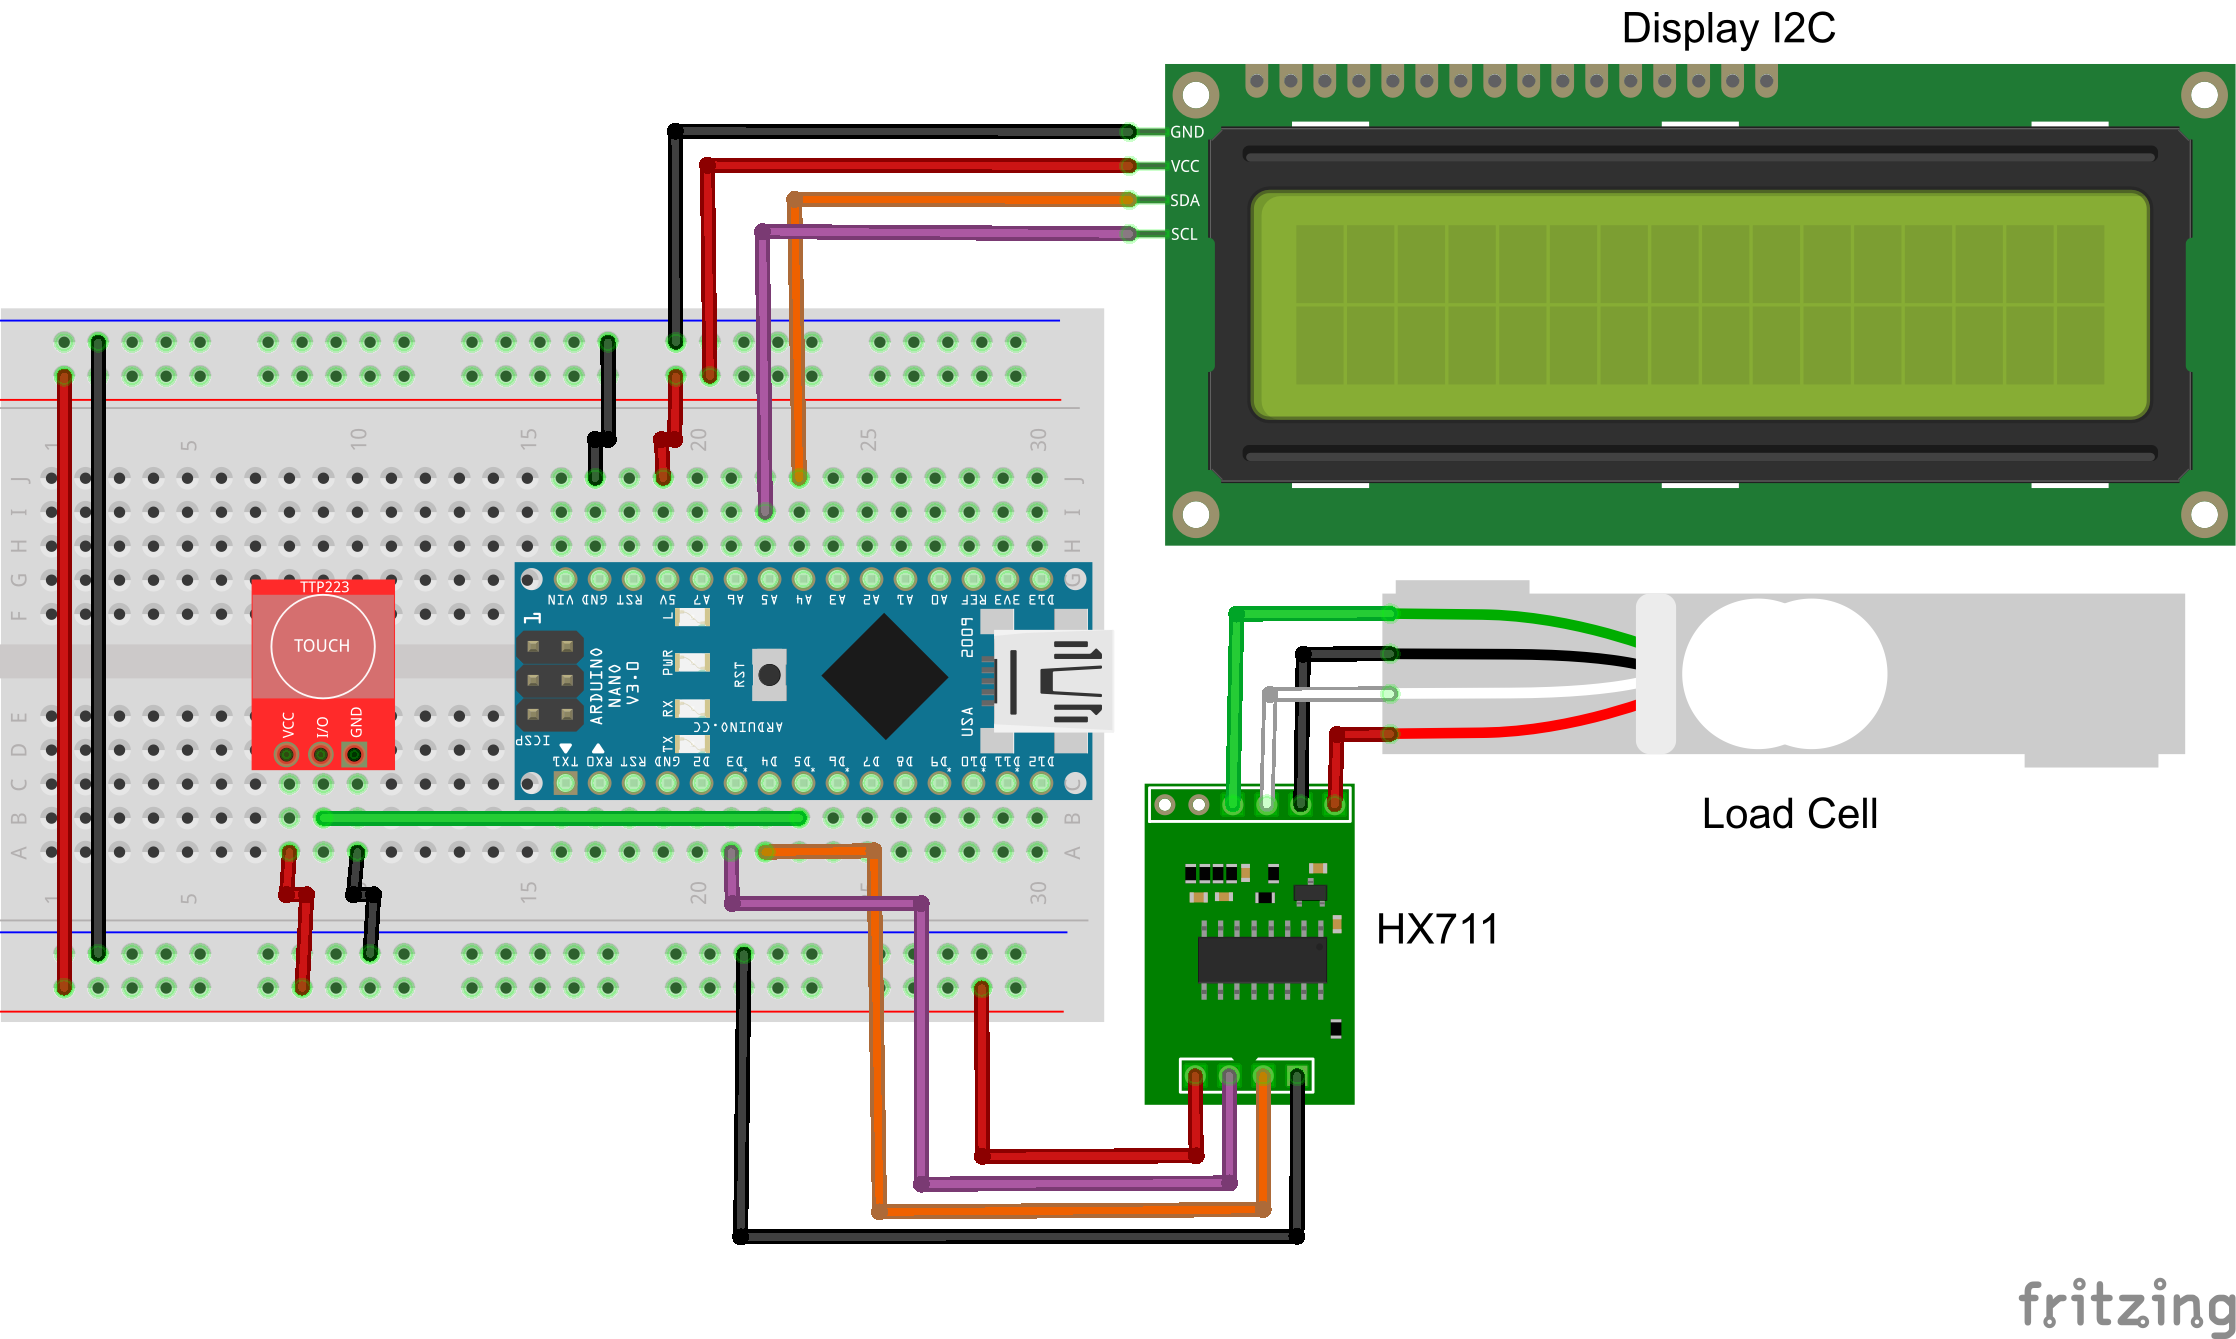
\includegraphics[width=\textwidth]{medias/load_cell_schematic_bb.png}
\caption{Schematic}
\end{figure}

\subsection{HX711 load cell amplifier}
\begin{itemize}
\item \texttt{LOADCELL\_DOUT\_PIN} is connected to pin 3 of the Arduino board.
\item \texttt{LOADCELL\_SCK\_PIN} is connected to pin 2 of the Arduino board.
\end{itemize}

\subsection{LCD display (I2C interface)}
\begin{itemize}
\item Address: 0x27
\item Columns: 16
\item Rows: 2
\end{itemize}

\subsection{Tare button}
\begin{itemize}
\item Connect one terminal of the button to a digital input pin of the Arduino board.
\item Connect the other terminal of the button to the ground (GND) pin of the Arduino board.
\item Optionally, add a pull-up resistor between the digital input pin and the 5V pin of the Arduino board to ensure stable button readings. (We implemented it, if you want to add it, you can modify it in declaration part)
\end{itemize}